\documentclass[12pt,a4paper]{ctexart}
\usepackage{geometry}
\geometry{left=2.5cm,right=2.5cm,top=2.5cm,bottom=2.5cm}
\usepackage{amsmath,amssymb}
\usepackage{booktabs}
\usepackage{graphicx}
\usepackage{hyperref}
\usepackage{xcolor}
\usepackage{array}
\usepackage{multirow}
\usepackage{enumitem}
\usepackage{longtable}
\usepackage{tcolorbox}
\tcbuselibrary{most}

\hypersetup{
  colorlinks=true,
  linkcolor=blue,
  citecolor=blue
}

\newtcolorbox{warningbox}[1][]{
  colback=red!5!white, colframe=red!60!black,
  fonttitle=\bfseries, title=#1,
  left=6pt, right=6pt, top=4pt, bottom=4pt
}

\newtcolorbox{infobox}[1][]{
  colback=blue!5!white, colframe=blue!60!black,
  fonttitle=\bfseries, title=#1,
  left=6pt, right=6pt, top=4pt, bottom=4pt
}

\title{\textbf{岗位综合性计算方法梳理}\\[0.5em]
\large 结构：目的-方法-结果-改进(可能性)}
\author{宋宇}
\date{2026年2月26}

\begin{document}
\maketitle
\tableofcontents
\newpage


% ===================================================================
\section{总览}
\label{sec:overview}
% ===================================================================

从代码溯源；梳理在计算岗位综合度的过程中每一步的目的和具体采用方法；从而进一步查找问题来源。

\subsection{核心流程}

\begin{verbatim}
原始招聘广告 (window_*.csv, ~860万条)
  |
  v
[Step 1] 文本预处理 (step1_preprocess.py)
  jieba分词 -> 停词过滤 -> bigram合并
  -> processed_corpus.jsonl (每行: id, year, tokens)
  |
  v
[Step 2] LDA模型训练 (step2_train_fast.py)
  10%采样 -> tomotopy LDA K=50 -> 1000轮Gibbs
  -> global_lda_fast.bin
  |
  v
[Step 3] 主题推断 + 熵计算 (step3_infer.py)
  贝叶斯folding-in -> 每条广告的50维主题分布
  -> Shannon entropy (香农熵 - 综合性主指标)
  -> HHI (辅助指标；虽然说算法不一样，但结果就是HHI = 1- shannon entropy)
  -> final_results_sample.csv
  |
  v
[稳健性检验] 
  +-- 词频熵 (compute_word_entropy.py): 不依赖LDA
  +-- SBERT技能指纹 (compute_skill_fingerprint.py): 20维
  +-- 早期gensim版本 (build_comprehensiveness_index.py)
\end{verbatim}


% ===================================================================
\section{Step 1：文本预处理}
\label{sec:step1}
% ===================================================================

\begin{itemize}[leftmargin=2em]
\item \textbf{代码}：\texttt{src/lda/step1\_preprocess.py}
\item \textbf{目的}：将原始CSV中的岗位描述文本转化为可供LDA训练的token序列。
\item \textbf{输入}：\texttt{data/processed/windows/window\_YYYY\_YYYY.csv}，
读取 \texttt{cleaned\_requirements} 列。
\item \textbf{输出}：\texttt{output/processed\_corpus.jsonl}，
每行JSON包含 \texttt{id}, \texttt{year}, \texttt{tokens}。
\end{itemize}

\subsection{具体方法}

\subsubsection{文本清洗}
\begin{enumerate}
\item 全文转换为小写格式。
\item 特殊词汇处理，以避免正则过滤后造成误解：\texttt{c++ $\to$ cpp}，\texttt{c\# $\to$ csharp}，\texttt{.net $\to$ dotnet}。 ($c++ $和$ c\# $会在正则后变成c，就会导致和c语言混淆；这里可能存在特殊词汇处理不够完善的问题)
\item 正则过滤：只保留中文字符（\texttt{\textbackslash u4e00-\textbackslash u9fa5}）和英文字母（\texttt{a-z}），
去除所有数字和标点符号。(数字保留下来会有变化吗？)
\end{enumerate}

\subsubsection{分词与过滤}
\begin{enumerate}
\item 使用jieba分词库（\texttt{jieba.lcut(text)}，精确模式）将连续的中文文本切分成一个个词语。\\
例如``熟练使用Python进行数据分析''会被切成``熟练/使用/Python/进行/数据/分析''。
\\jieba内部自带一个通用中文词典（约35万词条），
根据词典中已有的词和它们的使用频率来决定最优切分方式；
对于词典中没有的词（如新出现的专业术语），则用统计模型尝试猜测词的边界。
\\当前代码没有额外加载招聘领域的专业词典，
因此一些行业术语可能被错误切分（如``运维工程师''可能被切成``运维/工程师''或``运/维/工程师''）。
\\（其实有esco的行业术语词典来的，甚至部署到本地了，但是没有使用。。。这个肯定得改）
\item 停词过滤：约70个中文停用词（通用词 + HR泛化词），如
``职责''``任职''``要求''``负责''``具有''``熟悉''等。
\item 中文词：保留长度$\geq 2$的词（单字全部丢弃）。
\item 英文词：仅保留白名单中的9个编程语言名
（python, java, sql, c, r, go, cpp, csharp, dotnet），
其余英文词全部丢弃。

\textbf{问题}：经过对原始语料10\%采样统计（脚本 \texttt{scripts/count\_english\_token\_freq.py}），
共发现26,207个不同的英文token。当前白名单仅保留9个，
！但实际上大量有意义的跨行业英文词都被扔掉了：
\begin{itemize}
\item 办公/设计工具：office(38k), excel(30k), cad(29k), ppt(17k), photoshop(12k), autocad(9k), solidworks(5k)
\item 企业系统：erp(11k), sap(3k), plc(6k), mes(1.7k), crm(1.5k)
\item IT基础设施：linux(11k), mysql(8k), web(8k), html(7k), css(7k), oracle(7k)
\item AI/新兴技术：ai(7k), android(5k), vue(4k), react(1.7k)
\item 标准/资质：iso(7k), gmp(3k), cet(4k), iatf(1.8k)
\item 人力/商务：hr(2k), seo(1.9k)
\end{itemize}
但与此同时，数据里也还有大量噪声：
\begin{itemize}
\item HTML残留标签：br(408k), div(313k), p(292k), li(5k), nbsp(3k)
\item 英文逻辑连接词等虚词：and(7k), in(3k), to(3k), the(3k), of(3k), or(2k), with(2k)
\item 无意义的单字母：d(14k), b(11k), s(8k), a(6k), e(3k)等
\end{itemize}

\textbf{准备修改}
默认保留所有长度$\geq 2$的英文词，
仅用一个小黑名单排除HTML标签残留（br, div, nbsp, li, span, font, img, href, style, color, margin, padding等）
和英文虚词（and, the, in, to, of, or, with, for, is, are, be, an, at, by, on, as, it, we, do, if, no等）。
对单字母仅保留 c 和 r（编程语言）。
其余噪声交给 LDA 的 \texttt{min\_cf} 和 \texttt{rm\_top} 自动过滤。

\item 删除纯数字词。
\end{enumerate}

\subsubsection{Bigram合并（两遍扫描）}
\begin{enumerate}
\item Pass 1：遍历全部文档，统计相邻词对的共现频次。
参数：\texttt{BIGRAM\_MIN\_COUNT = 20}（最低共现20次），
\texttt{BIGRAM\_MAX\_PAIRS = 200,000}。
\item Pass 2：重新遍历文档，将频繁词对合并为 \texttt{词A\_词B} 格式
（贪心从左到右匹配）。
\end{enumerate}

\subsubsection{最终过滤}
\begin{itemize}
\item 文档token数 $<$ \texttt{MIN\_TOKENS = 5} 的记录被丢弃，不写入JSONL。
\end{itemize}

\subsection{结果}
\begin{itemize}
\item 输入：约860万条招聘广告。
\item 输出：\texttt{processed\_corpus.jsonl}，过滤后保留的文档数取决于
\texttt{MIN\_TOKENS}阈值。
\end{itemize}

\subsection{其他问题和可能改进}
\begin{enumerate}
\item \textbf{bigram是把所有年份混在一起统计的}：
代码扫一遍全部860万条数据，计算相邻两个词一起出现了多少次，达到20次就合并成一个词。
问题是：比如``大模型''这个词2022年之前根本没人提，
只有2023--2024年的JD里才会出现——
但频次是拿全部9年的数据一起算的，
如果``大模型''在最近两年只出现了十几次，没到20次的门槛，
它就不会被合并，jieba可能把它切成``大''和``模型''两个词。
（不过实际影响可能不大，860万条数据量很大，近两年的出现次数大概率能够20次）
\end{enumerate}


% ===================================================================
\section{Step 2：LDA模型训练}
\label{sec:step2}
% ===================================================================

\begin{itemize}[leftmargin=2em]
\item \textbf{代码}：\texttt{src/lda/step2\_train\_fast.py}
\item \textbf{目的}：基于Step 1输出的token序列，训练一个LDA主题模型——
让模型自己从860万条招聘广告里归纳出$K$个主题，
训练好的模型后面Step 3用于推断任意一条JD在这$K$个主题上的分布。
\item \textbf{输入}：\texttt{output/processed\_corpus.jsonl}
\item \textbf{输出}：\texttt{output/global\_lda\_fast.bin}（tomotopy模型文件）
\end{itemize}

\subsection{具体方法}

\begin{itemize}
\item 模型：用的是 \texttt{tomotopy} 这个Python库（底层是C++写的，比gensim快很多）。
\\训练算法是Gibbs sampling——
一开始随机给每个词分配一个主题，然后反复迭代1000轮，
\\每轮对每个词重新抽签决定它属于哪个主题，
抽签概率取决于这个词在哪个主题里更常见 以及 这条JD目前偏向哪个主题。
迭代够多次就收敛了，最终得到每个主题由哪些词组成。
\item 主题数：$K = 50$。(后续会讲为什么选50)
\item \textbf{采样训练}：只随机抽了10\%的文档来训练（\texttt{SAMPLE\_RATE = 0.1}，随机种子42），
也就是大约86万条，不是全部860万条。
原因是Gibbs sampling每轮要对每个词重新抽签，
860万条$\times$1000轮太多了，跑不动(非要跑也能跑，但是cpu占用率太高了，会卡住)；
其实LDA学的是``哪些词经常一起出现''这种统计规律，
86万条已经够多了，再加数据对主题词分布的改善很有限。
\item 迭代：1000轮Gibbs sampling（\texttt{ITERATIONS = 1000}）。
\item 词表过滤：
\begin{itemize}
\item \texttt{min\_cf = 10}：在训练集中出现少于10次的词被移除。
\item \texttt{rm\_top = 15}：移除频率最高的15个词。(因为它们在几乎所有JD里都会出现，对区分主题没有帮助——如果一个词在所有主题里都高频出现，LDA会把它均匀分配到所有主题里，相当于噪声，反而稀释了真正有区分度的词。)
\end{itemize}
\item 最小文档长度：过滤后token数 $<$ \texttt{MIN\_TOKENS = 5} 的文档不加入模型。
\item 并行：\texttt{workers = 0}（tomotopy默认使用所有CPU核心）。
\end{itemize}

\subsection{K的选择}

代码在这里：\texttt{scripts/k\_selection.py}。
\\分别试了 $K \in \{20, 30, 40, 50, 60, 70, 80, 100\}$，
每个K都跑了一遍完整的LDA训练（同样的10\%采样、1000轮），
然后算三个指标来比较哪个K最好：

\begin{itemize}
\item \textbf{ $C_V$ coherence}（主题连贯度）：
衡量每个主题里的top词是不是语义上相关的。越高越好。
\item \textbf{$U_{Mass}$ coherence}：
类似的思路，但用的是词的共现频率来算。越高越好。
\item \textbf{Log-likelihood per word}：
模型对数据的拟合程度。越高越好，但K越大这个值一定会涨（过拟合）。
\end{itemize}

实际结果（见表~\ref{fig:k_coherence}）：

\begin{table}[h]
\centering
\small
\begin{tabular}{cccc}
\toprule
K & C\_V & U\_Mass & LL/word \\
\midrule
20 & 0.575 & $-$4.27 & $-$9.74 \\
30 & 0.590 & $-$4.37 & $-$9.67 \\
40 & 0.588 & $-$4.57 & $-$9.62 \\
\textbf{50} & \textbf{0.597} & $-$4.62 & $-$9.58 \\
60 & 0.580 & $-$4.88 & $-$9.57 \\
70 & 0.588 & $-$4.81 & $-$9.55 \\
80 & 0.593 & $-$4.84 & $-$9.53 \\
100 & 0.557 & $-$5.51 & $-$9.53 \\
\bottomrule
\end{tabular}
\end{table}

$C_V$在$K=50$时最高（0.597），但$K=30$也有0.590，差距只有0.007，
看图上$C_V$那条线一直在锯齿形跳，这点差距基本可以视为噪声。
$U_{Mass}$的话$K=30$（$-4.37$）明显好于$K=50$（$-4.62$），而且$K$越大$U_{Mass}$越差。
LL/word随$K$增大单调上升，但这个指标$K$越大一定越高（过拟合也会涨），不太能单独用来选$K$。

所以纯看coherence指标的话，$K=30$和$K=50$其实差不多，甚至$K=30$的$U_{Mass}$更好。
当前选$K=50$更多是觉得860万条覆盖几百种职业，30个主题粒度可能太粗。
（但这个理由不够充分，感觉可以试试$K=30$也跑一遍看最终的entropy趋势有没有变化。

\begin{figure}[h]
\centering
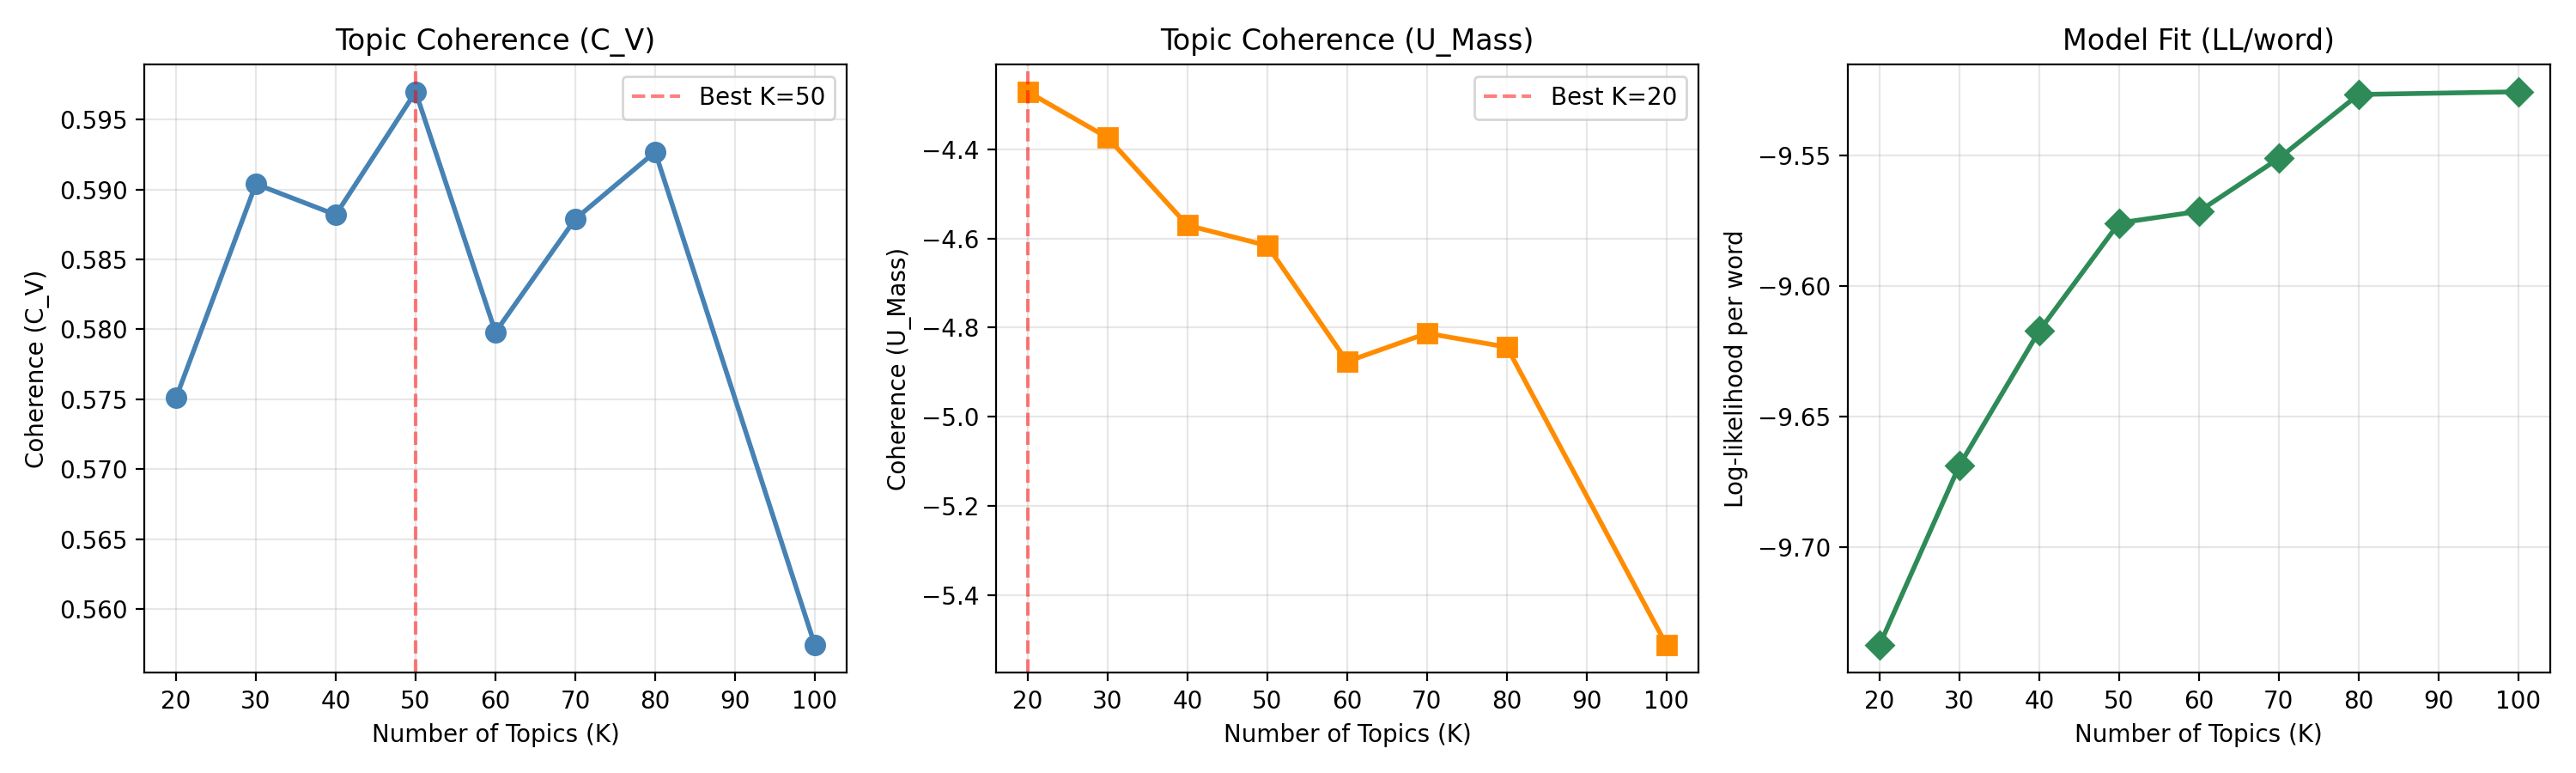
\includegraphics[width=0.95\textwidth]{k_coherence.png}
\caption{不同$K$值下的Coherence和模型拟合度。$K=50$是$C_V$的最高点。}
\label{fig:k_coherence}
\end{figure}

另外还做了敏感性分析（\texttt{scripts/k\_sensitivity.py}），
检验``就算$K$选错了，最终的entropy时间趋势会不会完全不一样''。
做法很简单：拿上面训练好的8个不同$K$的模型，分别对全量860万条JD做folding-in推断，
算出每年的平均entropy，然后把8条线画在一张图上看趋势是不是一致的。

\begin{figure}[h]
\centering
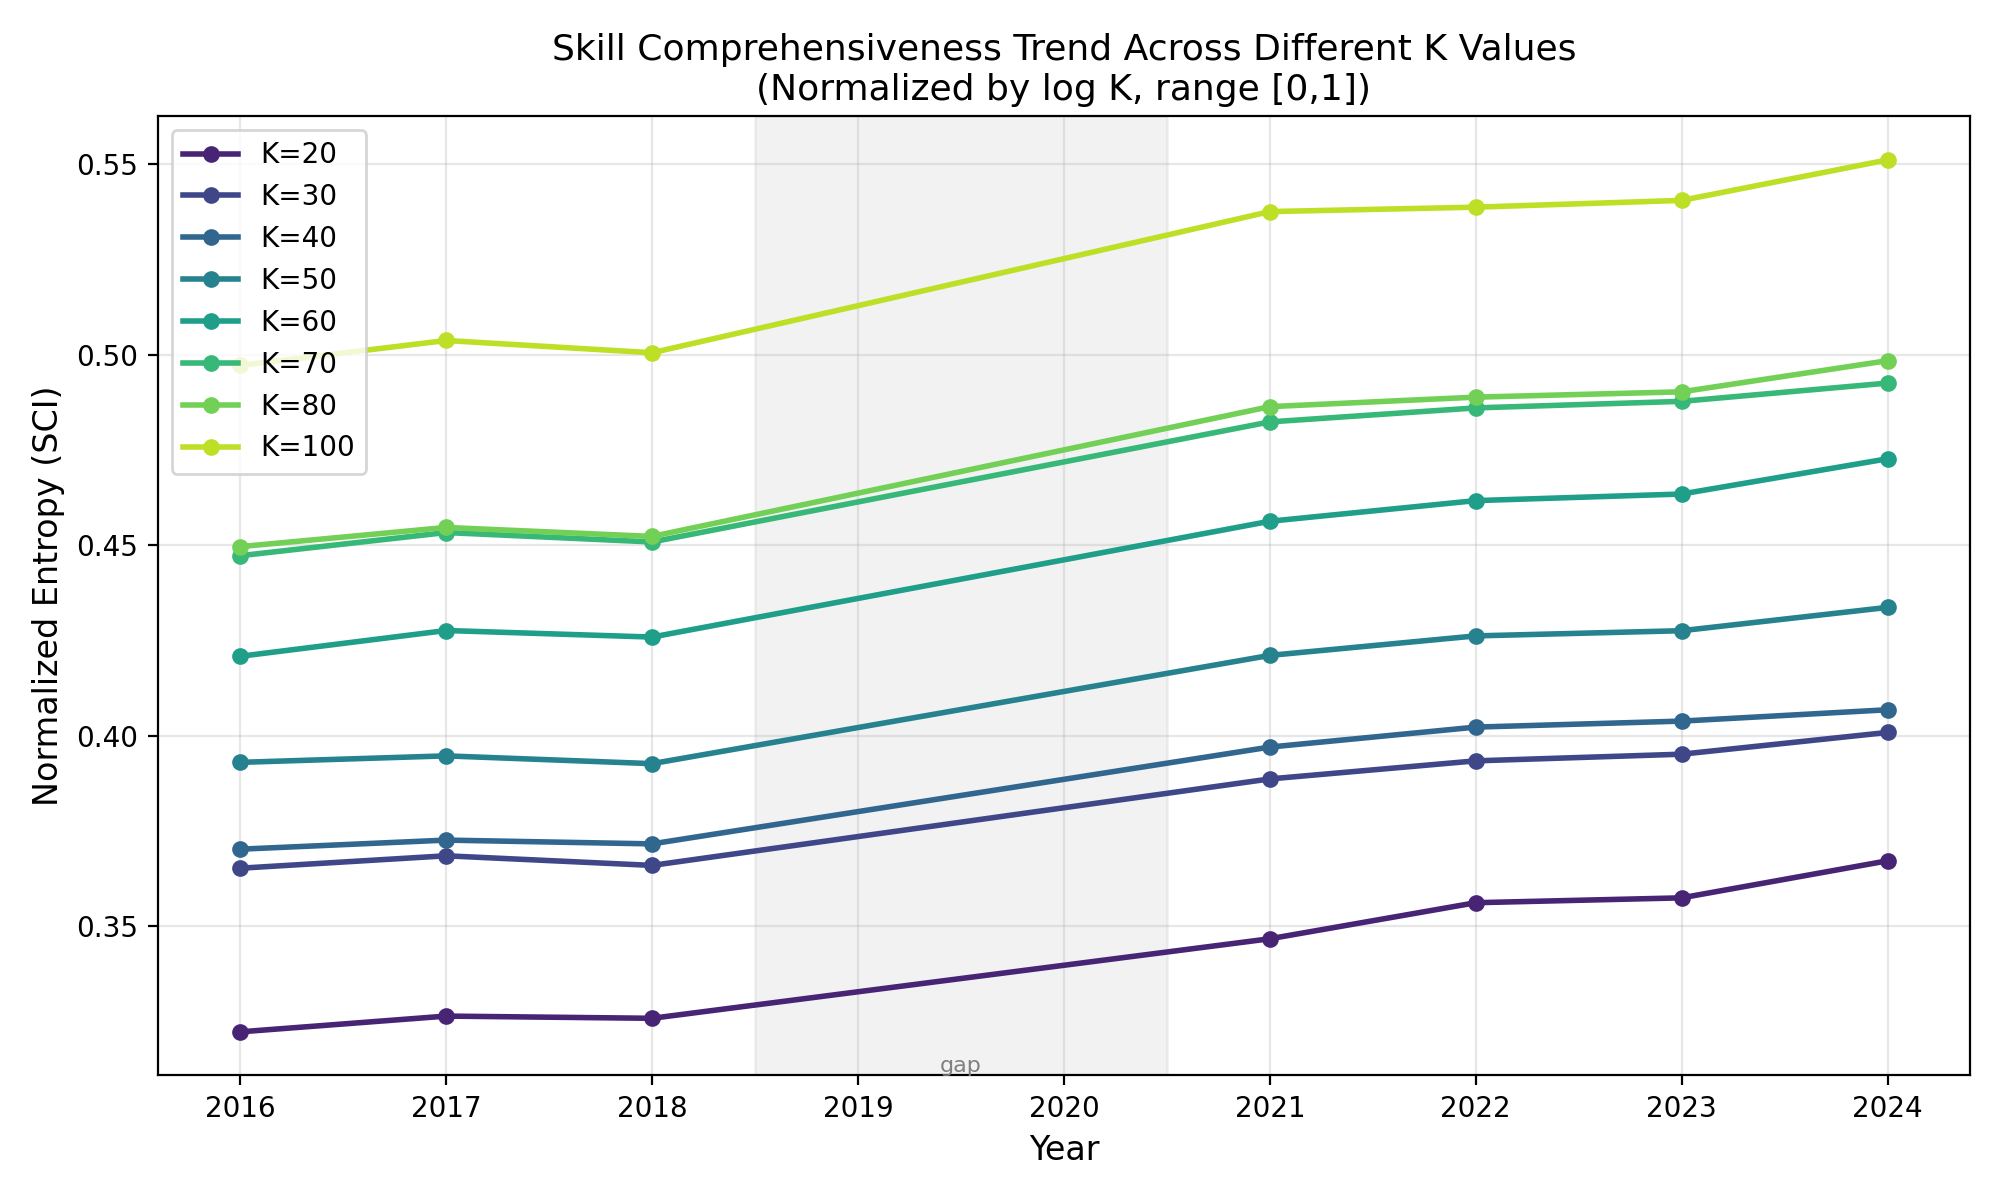
\includegraphics[width=0.85\textwidth]{k_sensitivity_trend.png}
\caption{不同$K$下的年度entropy趋势。8条线走向基本一致，都是逐年上升。
$K$越大entropy绝对值越高（因为主题多了分布更分散），但趋势方向不受$K$影响。
中间2019--2020的灰色区域是数据断层（那两年没有数据）。}
\label{fig:k_sensitivity_trend}
\end{figure}

还算了每个$K$下entropy对年份做OLS回归的斜率（图~\ref{fig:k_sensitivity_slope}），
斜率都是正的（每年涨$\sim$5--7$\times 10^{-3}$），
说明``岗位在变综合''这个趋势不管用哪个$K$都能看到，不是$K=50$碰巧出来的结果。

\begin{figure}[h]
\centering
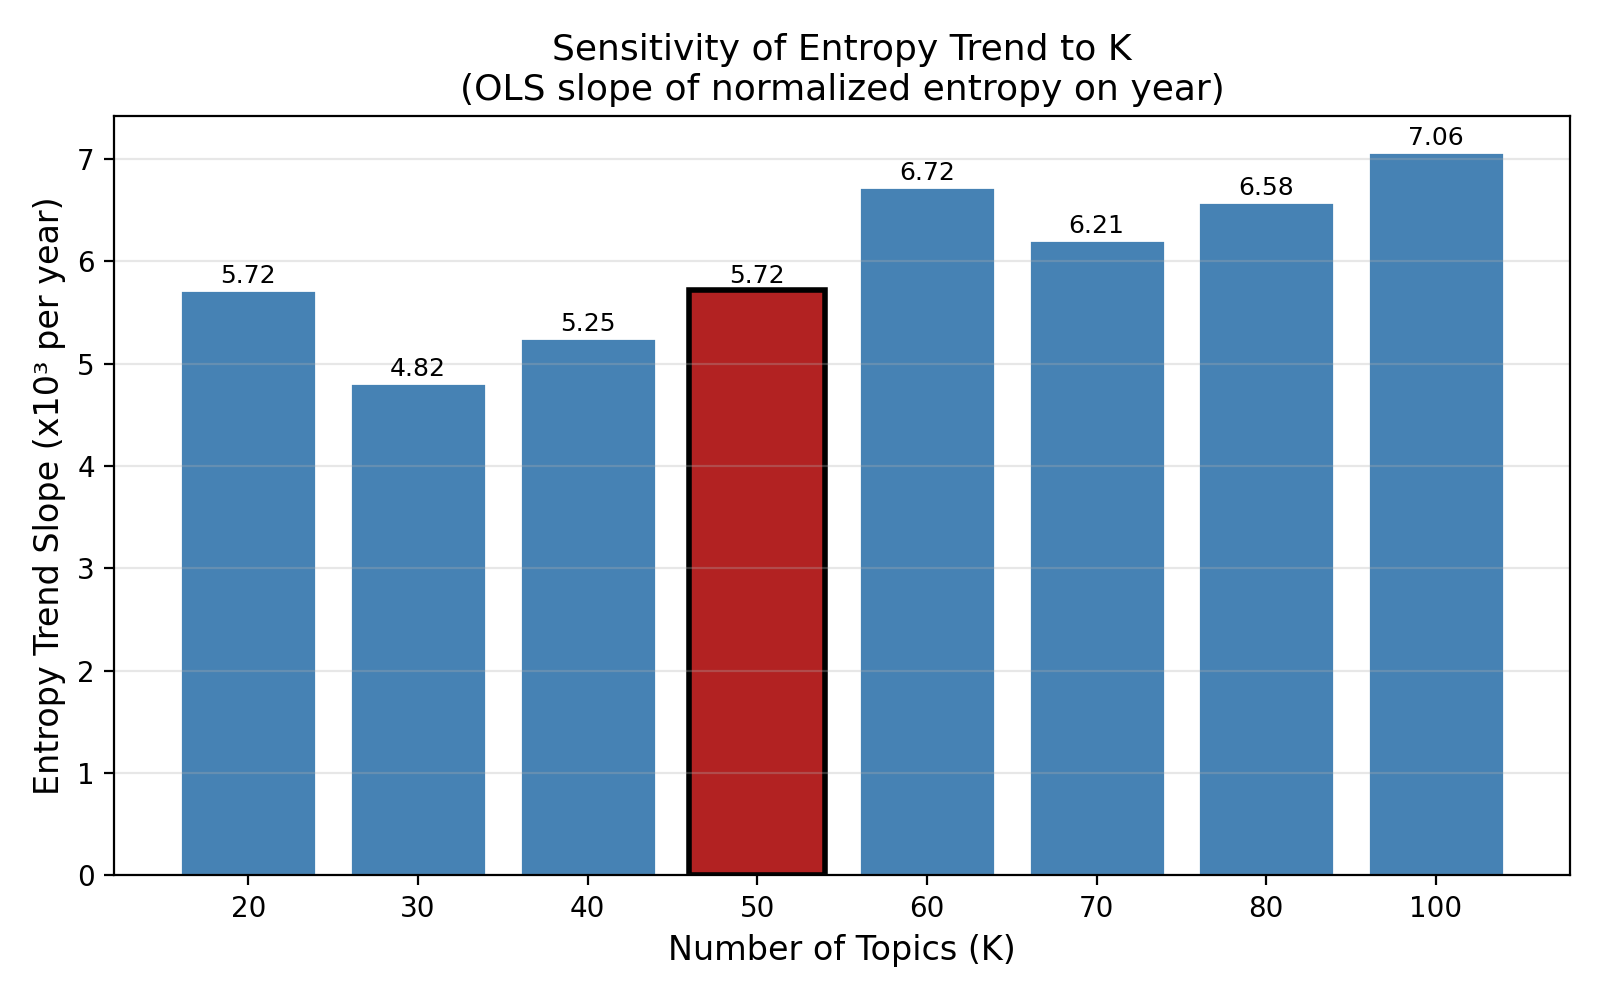
\includegraphics[width=0.7\textwidth]{k_sensitivity_slope.png}
\caption{不同$K$下entropy年趋势的OLS斜率。全部为正，$K=50$（红色）处于中间水平。}
\label{fig:k_sensitivity_slope}
\end{figure}

\subsection{结果}
\begin{itemize}
\item 输出模型文件 \texttt{global\_lda\_fast.bin}，
包含50个主题的词分布（$P(\text{word} \mid \text{topic})$矩阵）
和Dirichlet先验参数$\alpha$。
\end{itemize}




% ===================================================================
\section{Step 3：主题推断与综合性计算}
\label{sec:step3}
% ===================================================================

\begin{itemize}[leftmargin=2em]
\item \textbf{代码}：\texttt{src/lda/step3\_infer.py}
\item \textbf{目的}：Step 2只用了10\%的数据训练模型，
这一步是拿训练好的模型去给\textbf{全部}860万条JD算主题分布——
每条JD得到一个50维的向量（在50个主题上各占多少比例），
然后基于这个向量算出综合性得分（entropy越高=主题越分散=越综合）。
\item \textbf{输入}：Step 1的JSONL + Step 2的模型文件
\item \textbf{输出}：\texttt{output/final\_results\_sample.csv}，
每条JD一行，包含 entropy\_score、hhi\_score、dominant\_topic\_id、dominant\_topic\_prob
\end{itemize}

\subsection{具体方法}

\subsubsection{怎么从模型推断每条JD的主题分布}

Step 2训练的时候用的是Gibbs sampling（反复迭代抽签），
但推断860万条JD如果也用Gibbs的话太慢了。
所以这里用了一个快一些的方法(\textbf{解析法folding-in}——
不迭代，直接一步算出来。)

原理其实是概统的贝叶斯定理。
训练完的模型知道的是：``如果一条JD属于主题k，它出现某个词的概率是多少''，
即 $P(\text{词} \mid \text{主题})$。
但我们想知道的是反过来的：``看到这条JD里的这些词，它属于主题k的概率是多少''，
即 $P(\text{主题} \mid \text{词})$。
\[
P(\text{主题} \mid \text{这条JD的词}) \propto
P(\text{这条JD的词} \mid \text{主题}) \times P(\text{主题})
\]
右边第一项：把这条JD里每个词在主题k下的概率乘起来（模型训练时已经学到了）；
右边第二项：先验$\alpha$，就是``没看到任何词之前，你觉得每个主题的可能性有多大''。
两个乘一下，归一化让概率加起来等于1，就得到了这条JD在50个主题上的分布。
所以叫``解析法''——不需要像Gibbs那样迭代几百轮，直接一步乘法就出来了。
代价是精度可能不如Gibbs，尤其是词少的时候先验$\alpha$的影响会很大。

公式写出来就是：
\[
P(\text{topic}_k \mid \text{doc}) \propto \alpha_k \cdot \left[\prod_{w_i \in \text{doc}} P(w_i \mid \text{topic}_k)\right]^{1/n}
\]

实际代码里是用log算的（乘法变加法，避免数字太小溢出）：
\begin{enumerate}
\item 从训练好的模型里提取两个内容：
1. $K \times V$ 的词-主题概率矩阵（取log）； 2. 先验参数$\alpha$（取log）。
\item 对每条JD，把它的token在词表里找到对应的列。
不在词表里的词直接扔掉（这个后面讲问题）。
如果剩下的词不到5个就跳过这条JD。
\item 算分数：对这条JD里所有词的 $\log P(w_i \mid k)$ 取\textbf{平均值}（不是求和），
再加上 $\log \alpha_k$。
\item 做一个log-sum-exp归一化，让50个主题的概率加起来等于1。
\end{enumerate}

注意第3步取的是\textbf{mean}而不是标准的\textbf{sum}——
这不是LDA的标准写法，这里解释一下为什么不用sum：

假设一条JD有100个词，另一条只有10个词，而且它们用的词的分布完全一样。
如果用sum（把所有词的$\log P$加起来），100词那条加了100项，10词那条只加了10项，
前者的似然量级大得多，归一化之后主题分布会更尖锐（更集中在某几个主题上），
也就是说\textbf{长JD仅仅因为词多就会被判定为更``专业化''}。

用mean的话（加起来再除以词数），两条JD的结果是一样的——
消除了文档长度对结果的影响。
对我们的场景来说这可能更合理，
因为不同JD的长度差异很大（有的写了一大段，有的就几句话），
不希望长度本身影响综合性的判断。
但毕竟这不是标准做法，算是一个需要留意的点。

\subsubsection{综合性指标怎么算}

拿到50维主题分布之后，算综合性就相对比较技术了：

\paragraph{Shannon Entropy（主指标）：}

Shannon熵本来是信息论里的概念，衡量的是一个概率分布有多``不确定''。
核心是利用了 $f(x) = -x\log x$ 这个函数的形状：
它在$x=0$和$x=1$时都等于0，在中间（$x=1/e \approx 0.37$）达到最大值。
也就是说，一个概率项如果接近0（几乎不可能）或接近1（几乎确定），
它对entropy的贡献都很小；
只有概率处于``不上不下''的中间地带时，贡献才大。

Shannon熵就是把分布里每一项的 $-p_k \log p_k$ 加起来。
这样一来：
\begin{itemize}
\item 如果大部分概率集中在一两项上（其他项接近0），
那大部分项的贡献$\approx 0$，集中的那一项因为接近1贡献也不大，总和就小。
\item 如果概率均匀分散在很多项上（每项都处于中间值），
每一项都有不小的贡献，加起来总和就大。
\end{itemize}

放到我们的场景里就是：
一条JD的主题分布越``乱''（分散在很多主题上，你很难说它到底在讲什么），entropy越高；
越``集中''（大部分概率集中在一两个主题上，一看就知道在讲什么），entropy越低。

举个例子，假设只有3个主题：
\begin{itemize}
\item JD甲的主题分布是 $(1.0, 0, 0)$——100\%在主题1上，entropy $= 0$。
这条JD非常``专业化''，只讲一件事。
\item JD乙的主题分布是 $(0.33, 0.33, 0.33)$——均匀分布，entropy就比较大。
这条JD什么都沾一点，非常``综合化''。
\end{itemize}

公式：
\[
H = -\sum_{k=1}^{K} p_k \log p_k, \quad
H_{\text{norm}} = \frac{H}{\log K}
\]
除以$\log K$是为了归一化到$[0, 1]$区间（因为$K$个主题时最大熵就是$\log K$），
这样不管用$K=30$还是$K=50$，结果都在同一个尺度上可以比较。

\textbf{用entropy衡量综合性的几个隐藏问题：}

\begin{enumerate}
\item \textbf{行业构成变化（composition effect）}：
如果数据集里不同年份的行业比例在变
（比如2024年IT岗位的占比比2016年高了，而IT岗位本来entropy就偏高），
那年度平均entropy的上升趋势可能不是因为``每条JD变综合了''，
而是因为``本来entropy就高的行业占比变多了''。
光看平均值是分不清这两种情况的，
需要做行业内的对比（控制行业后看趋势还在不在）。

\item \textbf{噪声主题会压低entropy}：
如果50个主题里有一些是``垃圾主题''（招聘模板话术、HTML残留等），
归一化的分母还是$\log 50$，但有效的主题数可能只有40个。
这意味着entropy被系统性低估了——
而且如果噪声主题的占比随时间变化（比如早年HTML残留更多），
趋势本身也会被扭曲。

\item \textbf{JD长度可能逐年在变}：
近几年的招聘广告普遍比早年写得更详细（平台要求越来越规范、企业间竞争等），
就算用了mean消除了长度对folding-in的直接影响，
但词更多$\to$覆盖的主题词更广$\to$推断出来的主题分布可能更分散$\to$entropy更高。
也就是说entropy上升的趋势可能部分是JD变长导致的，
不完全是``技能真的变综合了''。
需要检查一下各年份的平均JD长度（token数），
如果确实在涨，可能需要在回归里控制文档长度。
\end{enumerate}

\paragraph{HHI指数（辅助指标）：}

HHI（Herfindahl-Hirschman Index）本来是经济学里衡量市场集中度的指标——
比如一个行业有几家公司，每家的市场份额是$p_k$，
HHI就是把每家的份额平方之后加起来：$\sum p_k^2$。
如果一家独大（$p_1 = 1$），HHI $= 1$（完全垄断）；
如果很多家平分市场（每家$p_k = 1/K$），HHI $= 1/K$（很小，很分散）。

核心是利用了$f(x) = x^2$的性质：平方会放大大的值、压缩小的值。
如果一项占了0.8，平方后是0.64，贡献很大；
如果一项只占0.05，平方后是0.0025，几乎可以忽略。
所以HHI本质上在数``有没有哪一项特别大''。

放到我们的场景里：把``公司市场份额''换成``主题占比''就行了。
\[
\text{HHI} = \sum_{k=1}^{K} p_k^2
\]
HHI越低=主题越分散=越综合；HHI越高=主题越集中=越专业。
和entropy度量的其实是同一件事，只是一个用$-x\log x$、一个用$x^2$，方向相反。

（代码输出的是原始HHI值，没有做$1 - \text{HHI}$的转换，所以HHI越\textbf{小}越综合）

\paragraph{主导主题：}
顺便记录了每条JD概率最高的那个主题（dominant\_topic\_id）和它的概率。
这个不用于计算综合性，但可以拿来看``某个行业的JD主要在讲什么主题''。

\subsubsection{并行化}
860万条一条一条算太慢，所以用了multiprocessing并行（最多8核），
每次丢10,000条给一个worker处理。
每个worker启动时加载一次模型、提取矩阵，然后就不再需要模型对象了。

\subsection{结果}
输出 \texttt{final\_results\_sample.csv}，
每条通过过滤的JD一行，有entropy\_score和hhi\_score两个综合性得分。

\subsection{改进可能性}
\begin{enumerate}
\item \textbf{folding-in对短JD不太友好}：
这个解析法比Gibbs快100倍以上，但有个问题——
如果一条JD只有几个词（比如刚好5个过了门槛），
那几个词提供的信息很弱，
推断出来的主题分布就会被先验$\alpha$拉着走，
变得很接近均匀分布，导致entropy偏高。
也就是说短JD可能被系统性地高估了综合性。

\item \textbf{不在词表里的词被默默扔掉了}：
如果一条JD用了很多低频专业术语（比如医学、法律领域的词），
这些词在Step 2训练时可能因为 \texttt{min\_cf=10} 被过滤掉了，
推断时就找不到它们，等于信息丢失了一部分。
极端情况下一条JD原本有20个词，过滤完只剩6个，那推断质量就很差。
\end{enumerate}


% ===================================================================
\section{辅助方法一：词频Shannon熵}
\label{sec:word_entropy}
% ===================================================================

\begin{itemize}[leftmargin=2em]
\item \textbf{代码}：\texttt{src/analysis/compute\_word\_entropy.py}
\item \textbf{目的}：做一个完全不依赖LDA的稳健性检验——
如果LDA的entropy说``岗位在变综合''，
那不用LDA、直接数词的多样性，能不能看到同样的趋势？
如果能，说明结论比较稳健；如果不能，说明可能是LDA本身的问题。
\item \textbf{输入}：原始CSV，重新分词（不用Step 1的JSONL）
\item \textbf{输出}：
\texttt{data/Heterogeneity/word\_entropy\_by\_id.csv}（每条JD一行）
和 \texttt{yearly\_word\_entropy\_stats.csv}（年度汇总）
\end{itemize}

\subsection{具体方法}

思路就是不管什么主题，
就看一条JD里用了多少不同的词、词的分布有多均匀。

\begin{enumerate}
\item 重新对原始文本做jieba分词（用和Step 1一样的清洗+分词逻辑）。
\item 加载Step 1生成的bigram集合，把经常连着出现的词对合并成一个词
（比如``数据''和``分析''合并成``数据\_分析''，和Step 1的处理保持一致）。
\item 用LDA模型的词表做过滤——只保留在LDA词表里出现过的token，
这样确保和主分析看的是同一批文档（token不到5个的JD同样跳过）。
\item 对每条JD，数每个词出现了几次，然后算词频熵：
\[
H_{\text{word}} = -\sum_{w} \frac{c_w}{n} \log \frac{c_w}{n} \bigg/ \log V
\]
$c_w$是词$w$在这条JD里出现的次数，$n$是总词数，$V$是不重复的词数。
除以$\log V$是归一化到$[0,1]$。

直觉上：如果一条JD反复只用几个词（比如一直说``沟通沟通沟通''），
少数词的频率很高、其他词频率接近0，词频熵就低；
如果用了很多不同的词且每个词出现差不多一样多次，词频熵就高。
\end{enumerate}

\subsection{和LDA熵的区别}

词频熵衡量的是``用了多少不同的词、词的分布有多均匀''（词汇多样性）；
LDA熵衡量的是``覆盖了多少不同的主题''（主题多样性）。
两者不是一回事——
一条JD可能用了很多不同的词（词频熵高），
但这些词可能都属于同一个主题（LDA熵低）。

\subsection{结果}

实际跑出来的年度平均词频熵：

\begin{table}[h]
\centering
\small
\begin{tabular}{ccc}
\toprule
年份 & 文档数 & 平均词频熵 \\
\midrule
2016 & 487,053 & 0.9973 \\
2017 & 872,174 & 0.9974 \\
2018 & 418,534 & 0.9972 \\
2021 & 1,236,730 & 0.9966 \\
2022 & 2,323,799 & 0.9961 \\
2023 & 1,243,166 & 0.9961 \\
2024 & 1,173,246 & 0.9962 \\
\bottomrule
\end{tabular}
\end{table}

（2019/2020数据量太少，2025是半年数据，这里不列了）

问题很明显：\textbf{所有年份的词频熵都在0.996--0.997之间，几乎没有区分度}。
原因是大部分JD里每个词只出现一次（unique\_tokens $\approx$ token\_count），
归一化之后词频熵直接就是1.0或接近1.0。

和LDA熵对比的话：LDA熵在0.3--0.7之间分布很广（有的JD很专业、有的很综合），
而词频熵全挤在0.996附近，基本分不出谁比谁更综合。
所以这个指标作为稳健性检验的价值有限——
不是说方法本身有错，而是招聘JD的文本特性（短文本、词很少重复）
导致词频熵天然就接近最大值，失去了区分能力。
(所以这个方法目前基本是废掉的)

\subsection{问题}
\begin{enumerate}
\item \textbf{区分度太低}：如上面的数据所示，0.9973 vs 0.9961这种级别的差异
很难说明什么问题，噪声可能比信号还大。
\item \textbf{对文档长度敏感}：
长JD几乎必然有更多不重复的词（Heaps' Law——词汇量随文档长度亚线性增长），
所以长JD的词频熵天然就高。
虽然除以了$\log V$做归一化（$V$本身也随长度增长），
能部分抵消长度效应，但抵消不完。
\end{enumerate}


% ===================================================================
\section{辅助方法二：SBERT技能指纹}
\label{sec:sbert}
% ===================================================================

\begin{itemize}[leftmargin=2em]
\item \textbf{代码}：\texttt{src/sbert/compute\_skill\_fingerprint.py}
\item \textbf{目的}：和LDA完全不同的思路做稳健性检验。
LDA是无监督的——让模型自己发现主题，我们不知道每个主题具体代表什么。
SBERT这边是有监督的——我们\textbf{事先定义好}20个技能维度（沟通、数据分析、编程……），
然后算每条JD和这20个维度各有多像，得到一个20维的``技能指纹''。
如果LDA和SBERT两种方法得出的综合性趋势一致，说明结论比较稳健。
\item \textbf{输入}：\texttt{data/processed/tokenized/window\_*\_tokenized.csv}
\item \textbf{输出}：
\texttt{output/sbert/fingerprint\_evolution\_TY.csv}（窗口级指纹）
和 \texttt{output/sbert/detail\_*.npy}（文档级相似度矩阵）
\end{itemize}

\subsection{具体方法}

\subsubsection{第一步：定义20个技能维度}

直接用了ESCO的标准技能分类，每个维度用一段中英文关键词来描述，比如：
\begin{itemize}
\item 1.1\_沟通技能：``沟通 表达 汇报 演讲 谈判 Communication Presentation...''
\item 2.3\_数据分析：``数据分析 统计 报表 SQL SPSS Excel Tableau...''
\item 8.1\_数字技术使用：``编程 开发 代码 Java C++ Python Linux Cloud...''
\item 9.1\_AIQ：``生成式 大模型 LLM AIGC ChatGPT Prompt Copilot...''
\end{itemize}
一共20个维度，覆盖沟通、团队协作、创造性思维、信息处理、数字素养、数据分析、
母语能力、外语能力、项目管理、人员管理、资源管理、体力要求、精细动作、
自主学习、适应能力、分析思维、决策能力、数字技术、软件应用、GenAI。

这20个维度是基于ESCO技能库的技能描述; 但是加入了9.1的AIQ，是最近看到的论文（AIQ（人工智能商数）: "一个人使用 AI 执行各种任务的能力。操作性定义为“一个人使用 AI 执行各种不同任务的能力”）
好处是每个维度的含义很明确、有国际标准背书，坏处是粒度固定，不一定完全适配中国劳动力市场。

而且像天宇老师说的，本文研究的正是AI是否让岗位变得更加综合了，更加综合就是它可能超越了之前的分类体系）

\subsubsection{第二步：用SBERT算相似度}

SBERT（Sentence-BERT）是一个预训练的语言模型，
能把一段文本变成一个固定长度的向量（embedding），
语义相似的文本向量也相似。
代码里用的是 \texttt{paraphrase-multilingual-MiniLM-L12-v2}，
一个支持中英文的小型模型。
（注意：代码注释里写的是 \texttt{BAAI/bge-large-zh-v1.5}，
但实际加载的是前面那个，最后还是以代码为准）

具体做法：
\begin{enumerate}
\item 把20个技能描述文本分别编码成20个向量。
\item 把每条JD的文本也编码成一个向量。
\item 算每条JD的向量和20个技能向量之间的余弦相似度——
余弦相似度就是两个向量夹角的余弦值，越接近1表示越相似。
这样每条JD就得到了一个20维的相似度向量，
比如$(0.4, 0.1, 0.05, ..., 0.3)$表示这条JD和``沟通''比较像（0.4），
和``数据分析''不太像（0.1），和``GenAI''比较像（0.3）。
\end{enumerate}

\subsubsection{第三步：AIQ维度的特殊处理}

因为AIQ是新兴的概念（2022年之前几乎没有），
SBERT可能会把一些并不真的在讲AI的JD也算出较高的相似度（误报）。
所以加了一个关键词门控：先在JD原文里数AIQ相关关键词出现了几次，
\begin{itemize}
\item 0次命中：相似度直接乘以0（不管SBERT算出来多高都归零）
\item 1次命中：乘以0.3
\item 2次命中：乘以0.6
\item 3次及以上：乘以1.0（保持原样）
\end{itemize}
这个映射关系是拍脑袋定的，没有理论依据，但意图是减少误报。

\subsubsection{第四步：算综合性}

拿到$N \times 20$的相似度矩阵之后，
和LDA熵的思路一样——把每条JD的20维相似度归一化成概率分布（让它们加起来等于1），
然后算Shannon熵：
\[
H_{\text{skill}} = -\sum_{d=1}^{20} q_d \log q_d \bigg/ \log 20
\]
值越高=技能覆盖越均匀=越综合。
（代码在 \texttt{src/analysis/build\_comprehensiveness\_index.py}
的 \texttt{calculate\_skill\_entropy()} 函数里）

窗口级指纹则是把这个窗口内所有JD的相似度矩阵按列取平均，
得到一个20维向量，代表这个时间段内``整体上哪些技能被提及得多''。

\subsection{问题}
\begin{enumerate}
\item \textbf{模型太小}：
\texttt{paraphrase-multilingual-MiniLM-L12-v2} 是一个参数量较小的多语言模型，
对中文的理解能力有限。
用更大的中文专用模型（比如 \texttt{BAAI/bge-large-zh-v1.5}）
可能效果更好，但也更慢。
\item \textbf{AIQ门控的任意性}：
0次$\to$0、1次$\to$0.3、2次$\to$0.6、3次及以上$\to$1.0，
这个映射其实是自定义的。为什么1次是0.3而不是0.5...
还有就是为什么只对AIQ做门控，其他维度不做？
这些选择都缺乏理论依据，如果要用在正式分析里需要解释...
\item \textbf{余弦相似度直接当概率用}：
余弦相似度的取值范围是$[-1, 1]$，
虽然通常是正的，但把它归一化成概率分布再算熵，
物理含义不如LDA的主题分布那么清晰。
\end{enumerate}


% ===================================================================
\section{最最最早期的版本：gensim LDA}
\label{sec:gensim}
% ===================================================================

代码在 \texttt{src/analysis/build\_comprehensiveness\_index.py}。

这是最早写的版本，用的是gensim的 \texttt{LdaMulticore}，$K = 60$。
现在主分析已经换成tomotopy了，这个版本留着只是做个记录。

最大的区别是：gensim版本是\textbf{按时间窗口分别训练一个独立的LDA模型}。
比如2016年的JD训练一个60主题的模型，2017年再训练一个——
问题在于，两个模型各自学出来的主题是完全不同的东西。
2016年的``主题3''可能是``数据分析''，2017年的``主题3''可能是``市场营销''，
它们只是碰巧编号一样而已。
所以你没法直接说``2016年主题熵0.6、2017年主题熵0.7，说明综合性提高了''——
因为这两个熵是在不同的主题空间下算的，不可比。

tomotopy版本的做法是训练一个全局模型（所有年份的JD一起训练），
这样50个主题在所有年份间是一致的，
不同年份算出来的熵才有可比性。

另外推断方式也不同：
gensim版本用的是 \texttt{get\_document\_topics()}，
这是gensim内部的推断方法（也是基于Gibbs sampling的）；
tomotopy版本用的是我们自己写的解析法folding-in（前面Step 3讲过的那个，一步乘法算出来的）。
解析法快很多，但精度可能不如Gibbs。
不过因为我们的目的是算年度均值趋势而不是单条JD的精确分布，
速度优先是合理的。

还有$K$值不同：gensim版本用了$K = 60$，tomotopy版本用了$K = 50$
（关于为什么选50，前面Step 2的K选择部分讲过了）。


% ===================================================================
\section{总结：从原始文本到综合性数字的完整路径}
\label{sec:summary}
% ===================================================================

最后把整条链路捋一遍：

\begin{longtable}{p{1.2cm}p{3.2cm}p{3.2cm}p{3cm}p{3.5cm}}
\toprule
\textbf{步骤} & \textbf{what} & \textbf{how} & \textbf{关键参数} & \textbf{问题/待改} \\
\midrule
\endhead

Step 1 &
原始CSV $\to$ 清洗好的token序列（JSONL） &
jieba分词 + 停词过滤 + bigram合并 &
MIN\_TOKENS=5; 英文黑名单过滤 &
单字全丢是否太激进？ESCO词典已部署但还没加载（得改） \\
\midrule

Step 2 &
token序列 $\to$ LDA主题模型 &
tomotopy，Gibbs sampling 1000轮 &
K=50; 10\%采样; min\_cf=10; rm\_top=15 &
K=30的coherence其实和50差不多(甚至更好)，可以试试；采样10\%可能影响词表覆盖 \\
\midrule

Step 3 &
token序列 + 模型 $\to$ 每条JD的主题熵 &
解析法folding-in（贝叶斯一步推断）+ 几何均值归一化 &
MIN\_TOKENS=5; 8进程并行 &
短文档先验影响大；组成效应和噪声主题 \\
\midrule

词频熵 &
原始CSV $\to$ 每条JD的词频熵 &
统计词频 $\to$ Shannon熵 $/ \log V$ &
MIN\_TOKENS=5 &
所有年份都在0.997附近，基本没有区分度（废了） \\
\midrule

SBERT &
分词后文本 $\to$ 20维ESCO技能指纹 &
SBERT编码 $\to$ 余弦相似度 $\to$ 归一化成概率 $\to$ 算熵 &
20个ESCO标准维度; GenAI门控 &
维度定义主观；余弦相似度直接用来当概率这一操作目前无法解释，但可以看看有没有相关的文献 \\
\bottomrule
\end{longtable}

\vspace{0.5em}

核心链条就是这样的：

\begin{center}
\textbf{原始招聘文本} $\xrightarrow{\text{Step 1: 分词清洗}}$
\textbf{token序列} $\xrightarrow{\text{Step 2: 训练LDA}}$
\textbf{50个主题的模型} $\xrightarrow{\text{Step 3: folding-in推断}}$
\textbf{每条JD的主题分布} $\xrightarrow{\text{Shannon熵归一化}}$
\textbf{综合性得分}
\end{center}

说白了就是：拿到一条招聘广告，先切成词，然后问模型``这条JD涉及哪些主题、各占多少''，
最后看这个分布有多均匀——越均匀说明这条JD覆盖的主题越多，岗位越综合。

每一步都有可以质疑的地方（前面各节都讲了），误差会逐步传递。
所以后续还得要排查：哪些因素本身随时间在变（JD长度、行业组成等），
有没有在entropy趋势里制造假信号。


\end{document}
